\documentclass[12pt,a4paper]{article}
\usepackage[brazil]{babel}
\usepackage[utf8]{inputenc}
\usepackage[T1]{fontenc}
\usepackage{timbre-ic}
\usepackage{booktabs}
\usepackage[table]{xcolor}
\usepackage{url}
\usepackage{array}
\usepackage{graphicx}
\usepackage{pifont}
\usepackage{float}
\usepackage{multirow}
\usepackage{indentfirst}
\usepackage{afterpage}
\usepackage{paralist}
\usepackage{tabto}
\setlength{\parindent}{0mm}


\begin{document}

\markright{Diagrama de Classes}

\begin{titlepage}
\begin{center}
{\huge \textbf{Universidade Estadual de Campinas}}\\[0.2cm]
{\huge \textbf{Instituto de Computação}}\\[0.2cm]
%{\large Nome do departamento}\\[0.2cm]
{\large Ciência da Computação/Engenharia da Computação}\\[0.2cm]
{\large MC426A - Engenharia de Software / MC436A - Introdução à Engenharia de Software}\\[5.1cm]
{\bf \huge Diagrama de Classes - Modelagem Estática e Modelagem Dinâmica}\\[5.1cm]
\end{center}
{\large Alunos:\\
Heitor Siqueira --- RA 119532\\
Pedro Emílio Machado de Brito --- RA 137264\\
Vinícius Andrade Frederico --- RA 139223}\\[0.7cm]
{\large Professora: Ariadne Maria B. Rizzoni Carvalho}\\[1.5cm]
\begin{center}
{\large Campinas}\\[0.2cm]
{\large 2014}
\end{center}
\end{titlepage}

%%\vskip 15mm

\tableofcontents
\afterpage{\cfoot{\thepage}}

\newpage
%\pagestyle{plain}
%\pagenumbering{arabic}

% ------------------------------------------------------------------------------
% INTRODUCTION
% ------------------------------------------------------------------------------
\section{Introdução}
Este documento detalha a elaboração do diagrama de classes referente ao sistema \verb|CompreFacil.com|.
O documento de requisitos e o documento de casos de uso foram utilizados como base no detalhamento desta etapa.
A análise se deu apenas sobre o \textit{workflow} principal de compra, utilizando os casos de uso referentes a ``Navegação no Site, ``Compra de Produto'', ``Realizar Pagamento'' e ``Envio de Produto''.

\section{Classes Candidatas e Classes Eliminadas}
Como a análise foi restrita aos casos de uso previamente citados, alguns substantivos como Administrador e Atendente foram desconsiderados para o diagrama de classes.
As classes candidatas resultantes estão listadas a seguir.

\NumTabs{3}
\begin{inparaenum}
\item Site
\tab\item Correio
\tab\item Entrega
\tab\item Controle de Estoque
\tab\item Controle de Compras
\tab\item Produto
\tab\item Carrinho
\tab\item Compra
\tab\item Pagamento
\tab\item Cliente
\tab\item Intermediador
\end{inparaenum}\\

Alguns substantivos foram eliminados do diagrama por não justificarem a criação de uma nova classe.
Estes substantivos foram implementados como atributos nas classes já elaboradas.

\NumTabs{3}
\begin{inparaenum}
\item Endereço
\tab\item Identificador de cliente
\tab\item CPF
\tab\item Senha
\tab\item Itens no Carrinho
\tab\item Preço
\tab\item Tipo de Pagamento
\tab\item Tipo de Entrega
\tab\item Valor de Frete
\end{inparaenum}

\section{Diagrama MVC}
Com base nas classes e atributos desenvolvidos, foi gerado um diagrama de classes preliminar.
O padrão Model-View-Controller também foi aplicado sobre este diagrama, resultando na criação de uma nova classe \textit{Controle de Carrinho} para facilitar o gerenciamento das ações sobre o carrinho de compras.
\begin{figure}[h!]
\centering
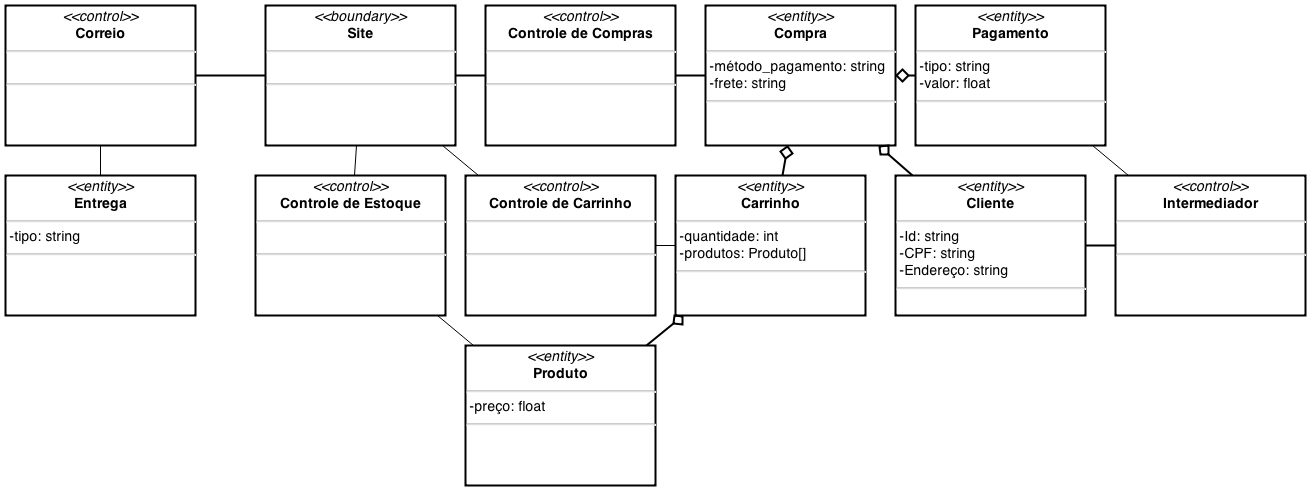
\includegraphics[width=0.85\textwidth]{img/MVC}
\caption{Diagrama MVC preliminar}
\end{figure}
\section{Eventos de Sistema}
Para elaboração dos eventos de sistema, foi considerado que o cliente possui cadastro e já está autenticado no site do sistema.
Os eventos resultantes estão listados a seguir:

\NumTabs{3}
\begin{inparaenum}
\item Buscar Produto
\tab\item Adicionar ao Carrinho
\tab\item Realizar Pagamento
\tab\item Confirmar Compra
\tab\item Alterar Estoque
\tab\item Enviar Produto
\end{inparaenum}



\section{Diagramas de Sequência}
Os diagramas a seguir são resultantes dos casos de uso relacionados a uma compra realizada pelo Cliente.
São referentes aos processos de busca no site, adicionar produtos ao carrinho do cliente, realizar e confirmar o pagamento de uma compra e liberar o envio de produtos no correio.

\begin{figure}[h!]
\centering
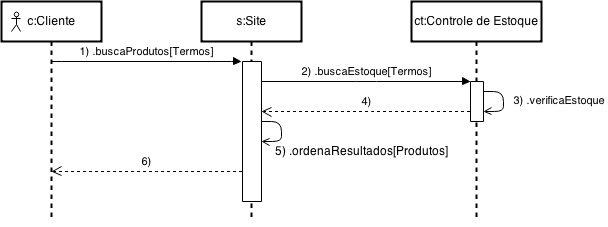
\includegraphics[width=0.85\textwidth]{img/sequencia_busca}
\caption{Busca no Site}
\end{figure}
\begin{figure}[h!]
\centering
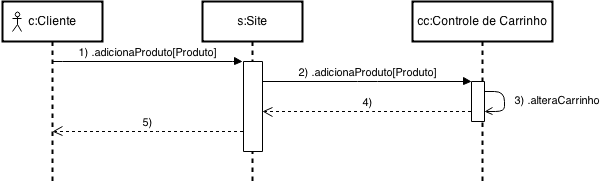
\includegraphics[width=0.85\textwidth]{img/sequencia_carrinho}
\caption{Adicionar Produtos ao Carrinho}
\end{figure}
\begin{figure}[h!]
\centering
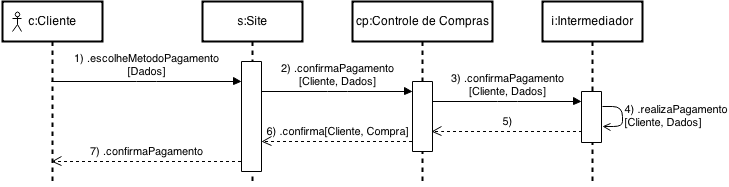
\includegraphics[width=0.9\textwidth]{img/sequencia_pagamento}
\caption{Realizar Pagamento}
\end{figure}
\begin{figure}[h!]
\centering
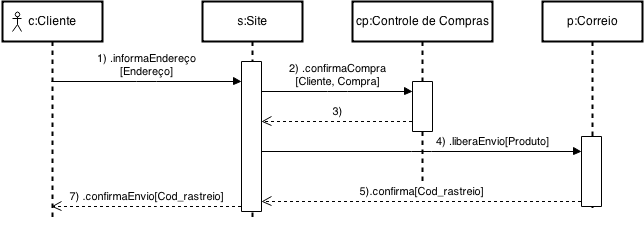
\includegraphics[width=0.85\textwidth]{img/sequencia_envio}
\caption{Confirmar envio de Compra}
\end{figure}

\section{Diagrama de Colaboração}

\section{Diagrama de Classes}

\section{Bibliografia}
    %\bibliographystyle{acm}
    %\bibliography{Documento_Extracao_Requisitos}
[1]  Rizzoni, Ariadne M. B. e Chiossi, Thelma C. dos Santos. Introdução à Engenharia de Software. Editora da Unicamp, 2001.\\

[2]  Sommerville, Ian. Software Engineering. Pearson, 2010.\\
\end{document}
